% Answer key for the Module 1 pen-and-paper sheet.
% Compile with: xelatex -interaction=nonstopmode solutions.tex   (run twice)
%
% It carries the questions as well as the answers, so it can be read on its
% own, and it draws the same figures as the sheet out of mapkit.tex -- an
% answer to a question about a map should be a map, and the route the student
% was asked to draw is the one thing a list of numbers cannot show them.
\documentclass[a4paper, 11pt]{extarticle}
\usepackage[top=0.7in, bottom=0.7in, left=0.8in, right=0.8in]{geometry}
\usepackage{amsmath}
\usepackage{amssymb}
\usepackage{array}
\usepackage{graphicx}
\usepackage{tcolorbox}
\usepackage{enumitem}
\usepackage{etoolbox}
\usepackage{tikz}
\usepackage{fontspec}
\usetikzlibrary{calc,positioning}
\definecolor{pltblue}{HTML}{1F77B4}

\IfFontExistsTF{Charter}{\setmainfont{Charter}}{
  \IfFontExistsTF{Iowan Old Style}{\setmainfont{Iowan Old Style}}{
    \IfFontExistsTF{Georgia}{\setmainfont{Georgia}}{}}}

\newcommand{\ppfont}{}
\IfFontExistsTF{Pretty Neat}{\renewcommand{\ppfont}{\fontspec{Pretty Neat}}}{
  \IfFontExistsTF{Humor Sans}{\renewcommand{\ppfont}{\fontspec{Humor Sans}}}{
    \IfFontExistsTF{Excalifont}{\renewcommand{\ppfont}{\fontspec{Excalifont}}}{}}}

\setlength{\parindent}{0pt}
\setlength{\parskip}{0.4em}
\raggedbottom

\newcommand{\parthead}[2]{%
  \vspace{0.5em}
  {\large\bfseries Part #1 --- #2}\par
  \vspace{-0.4em}\rule{\textwidth}{0.8pt}\par
  \vspace{0.2em}}

\newcolumntype{C}[1]{>{\centering\arraybackslash}p{#1}}

% An answer, set apart from the question it belongs to. Wrapped rather than
% switched: a bare \color inside a p-column cell costs the cell its first line.
\newcommand{\ans}[1]{\textbf{\textcolor{pltblue!75!black}{#1}}}

% The line that turns from question to answer.
\newcommand{\arrow}{\textcolor{pltblue!75!black}{$\Rightarrow$}\;}

% The maps and the figures, shared with exercise.tex.
% The maps and the single-city figures for the Module 1 sheet, kept in their
% own file because the answer key draws exactly the same maps with the
% circles filled in. Needs tikz, its calc and positioning libraries, and the
% colour pltblue, all of which the including file sets up.
% ---------------------------------------------------------------------------
% The map: seven Upstate New York highways over four cities. The cities sit
% where they really sit --- Ithaca west, Syracuse north, Binghamton south,
% Albany far east --- and every road on it is a road you can drive, so the
% figure reads as a road map rather than as an abstract graph. The degrees are
% Ithaca 3, Syracuse 4, Binghamton 4, Albany 3; US-11, on the second copy,
% takes Syracuse and Binghamton to 5.
%
% \nymap{extra roads}{numbers already filled in}. The route is written on the
% map, not copied out as letters: each road carries a circle, and the order it
% is driven goes in the circle.
% ---------------------------------------------------------------------------
\tikzset{
  % Every road is drawn the same, so no line weight or colour suggests a
  % distinction that isn't there. Only the shields differ, as on a real map.
  road/.style     = {line width=3.6pt, black!62, line cap=round},
  ishield/.style  = {draw=pltblue!60!black, fill=pltblue, text=white,
                     font=\bfseries\scriptsize, rounded corners=1.6pt,
                     inner sep=2pt},
  nshield/.style  = {draw=black!65, fill=white, text=black,
                     font=\bfseries\scriptsize, rounded corners=1.6pt,
                     inner sep=2pt},
  city/.style     = {circle, fill=black, inner sep=0pt, minimum size=6.5pt},
  cityname/.style = {font=\bfseries, inner sep=3pt},
  % The circle a student writes the order into, and the pre-filled number.
  ord/.style      = {circle, draw=pltblue!75, line width=0.7pt, fill=white,
                     minimum size=0.44cm, inner sep=0pt},
  ordnum/.style   = {font=\bfseries\footnotesize, inner sep=0pt},
}
\newcommand{\nymap}[2]{%
\begin{tikzpicture}[x=0.88cm, y=0.88cm]
    \begin{scope}
        \clip (0,0) rectangle (13,7.0);
        \fill[black!3] (0,0) rectangle (13,7.0);
        \fill[pltblue!22] (0,5.0) .. controls (1.8,6.0) and (2.6,6.5) ..
                          (5.0,7.0) -- (0,7.0) -- cycle;
    \end{scope}
    \node[font=\itshape\scriptsize, black!45, rotate=20] at (1.6,6.0)
        {Lake Ontario};

    \coordinate (I) at (1.8,2.3);
    \coordinate (S) at (5.0,5.9);
    \coordinate (B) at (4.4,0.9);
    \coordinate (A) at (11.6,3.3);

    \draw[road] (I) to[bend left=28]  (S);
    \draw[road] (I) to[bend right=26] (S);
    \draw[road] (I) to[bend right=8]  (B);
    \draw[road] (S) to[bend left=12]  (B);
    \draw[road] (S) to[bend left=8]   (A);
    \draw[road] (B) to[bend left=11]  (A);
    \draw[road] (B) to[bend right=11] (A);
    #1

    % Shields on a second pass, so no road is drawn across a number. Each
    % carries its circle as a label, on whichever side is clear of other roads.
    \path (I) to[bend left=28]  node[nshield, pos=0.55,
          label={[ord, name=o34]180:{}}] {NY-34} (S);
    \path (I) to[bend right=26] node[nshield, pos=0.35,
          label={[ord, name=o13]0:{}}]   {NY-13} (S);
    \path (I) to[bend right=8]  node[nshield, pos=0.50,
          label={[ord, name=o79]180:{}}] {NY-79} (B);
    \path (S) to[bend left=12]  node[ishield, pos=0.72,
          label={[ord, name=o81]90:{}}]  {I-81}  (B);
    \path (S) to[bend left=8]   node[ishield, pos=0.46,
          label={[ord, name=o90]90:{}}]  {I-90}  (A);
    \path (B) to[bend left=11]  node[ishield, pos=0.50,
          label={[ord, name=o88]90:{}}]  {I-88}  (A);
    \path (B) to[bend right=11] node[nshield, pos=0.50,
          label={[ord, name=o7]270:{}}]  {NY-7}  (A);

    \node[city] at (I) {};  \node[cityname, below left] at (I) {Ithaca};
    \node[city] at (S) {};  \node[cityname, above] at (S) {Syracuse};
    \node[city] at (B) {};  \node[cityname, below] at (B) {Binghamton};
    \node[city] at (A) {};  \node[cityname, above] at (A) {Albany};

    \draw[->, black!50, line width=1pt] (12.4,5.6) -- (12.4,6.35);
    \node[font=\bfseries\footnotesize, black!50] at (12.4,6.65) {N};
    \draw[black!35] (0,0) rectangle (13,7.0);
    #2
\end{tikzpicture}}

% US-11, the eighth road on the second copy. It really does run beside I-81,
% but it is bowed east far enough that both roads, and both shields, are
% legible; the shield is nudged clear of I-81's lane.
\newcommand{\usroad}{%
    \draw[road] (S) to[bend left=40] (B);
    \path (S) to[bend left=40] node[nshield, pos=0.50, xshift=17pt,
          label={[ord, name=o11]0:{}}] {US-11} (B);}

% ---------------------------------------------------------------------------
% One city on its own, with #1 road-ends radiating out. #2 takes extra TikZ so
% the k=2 figure can ship with its pairing already drawn.
% ---------------------------------------------------------------------------
\newcommand{\landdeg}[2]{%
\begin{tikzpicture}[x=1cm, y=1cm]
    \path (-1.55,-1.55) rectangle (1.55,1.55);
    \foreach \i in {1,...,#1} {
        \pgfmathsetmacro\ang{90 - (\i-1)*360/#1}
        \draw[line width=2.6pt, black!72] (\ang:0.38) -- (\ang:1.18);
        \draw[thick, fill=white] (\ang:1.28) circle (0.1);
    }
    \draw[thick, fill=white] (0,0) circle (0.38);
    #2
\end{tikzpicture}}

% ---------------------------------------------------------------------------
% The three graphs the sheet asks about after the map: Konigsberg as Euler
% drew it, the five bus stops, and the four-node network Part 3 predicts.
% ---------------------------------------------------------------------------
\newcommand{\konigsberggraph}{%
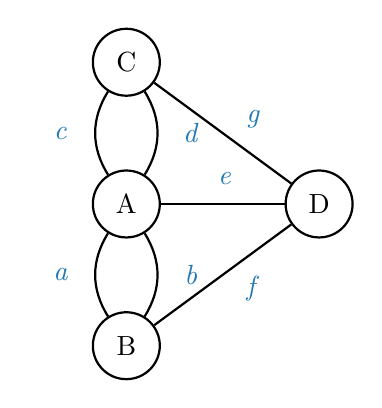
\begin{tikzpicture}[x=0.72cm, y=0.72cm, thick,
                    every node/.style={draw, circle, minimum size=0.85cm,
                                       inner sep=1pt, fill=white}]
    \node (C) at (0,2.5)   {C};
    \node (A) at (0,0)     {A};
    \node (B) at (0,-2.5)  {B};
    \node (D) at (3.4,0)   {D};
    \draw (A) to[bend left=32]  (B);
    \draw (A) to[bend right=32] (B);
    \draw (A) to[bend left=32]  (C);
    \draw (A) to[bend right=32] (C);
    \draw (A) -- (D);
    \draw (B) -- (D);
    \draw (C) -- (D);
    \node[draw=none, fill=none, pltblue] at (-1.15,-1.25) {\emph{a}};
    \node[draw=none, fill=none, pltblue] at ( 1.15,-1.25) {\emph{b}};
    \node[draw=none, fill=none, pltblue] at (-1.15, 1.25) {\emph{c}};
    \node[draw=none, fill=none, pltblue] at ( 1.15, 1.25) {\emph{d}};
    \node[draw=none, fill=none, pltblue] at ( 1.75, 0.45) {\emph{e}};
    \node[draw=none, fill=none, pltblue] at ( 2.25,-1.5)  {\emph{f}};
    \node[draw=none, fill=none, pltblue] at ( 2.25, 1.5)  {\emph{g}};
\end{tikzpicture}}

\newcommand{\busstopgraph}{%
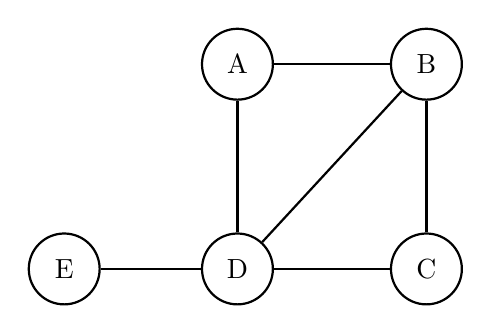
\begin{tikzpicture}[x=1cm, y=1cm, thick,
                    every node/.style={draw, circle, minimum size=0.9cm,
                                       inner sep=1pt, fill=white}]
    \node (A) at (0,1.6)   {A};
    \node (B) at (2.4,1.6) {B};
    \node (C) at (2.4,-1)  {C};
    \node (D) at (0,-1)    {D};
    \node (E) at (-2.2,-1) {E};
    \draw (A) -- (B);
    \draw (B) -- (C);
    \draw (C) -- (D);
    \draw (D) -- (A);
    \draw (B) -- (D);
    \draw (D) -- (E);
\end{tikzpicture}}

\newcommand{\fournodegraph}{%
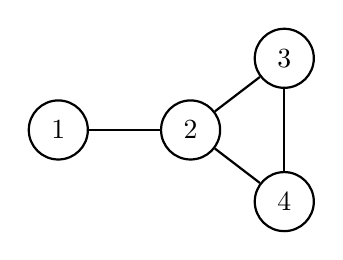
\begin{tikzpicture}[x=0.7cm, y=0.7cm, thick,
                    every node/.style={draw, circle, minimum size=0.75cm,
                                       inner sep=1pt, fill=white}]
    \node (1) at (-2.4,0)  {1};
    \node (2) at (0,0)     {2};
    \node (3) at (1.7,1.3) {3};
    \node (4) at (1.7,-1.3){4};
    \draw (1) -- (2);
    \draw (2) -- (3);
    \draw (2) -- (4);
    \draw (3) -- (4);
\end{tikzpicture}}


% The drive of 1(a), written into the circles of whichever map is drawn.
\newcommand{\tourfill}{%
  \node[ordnum] at (o13) {1};
  \node[ordnum] at (o34) {2};
  \node[ordnum] at (o79) {3};
  \node[ordnum] at (o81) {4};
  \node[ordnum] at (o90) {5};
  \node[ordnum] at (o88) {6};
  \node[ordnum] at (o7)  {7};}

% One "in here, out there" pairing on a single-city figure. The loop leaves and
% arrives along the bisector of the two road-ends, which is the one direction
% that always takes it clear of the city rather than across it.
\newcommand{\pairarc}[3][1.35]{%
  \pgfmathsetmacro{\pairmid}{(#2 + #3) / 2}%
  \draw[pltblue, dashed, line width=1.1pt]
    (#2:1.28) to[out=\pairmid, in=\pairmid, looseness=#1] (#3:1.28);}

\begin{document}

\begin{center}
{\ppfont\LARGE Answers}
\end{center}

{\small The sheet with its answers, \ans{in blue}. Question 1(a) has many right
answers and one of them is drawn; every other question has one.}

\parthead{1}{Seven highways}

Seven highways join four Upstate New York cities: Ithaca, Syracuse,
Binghamton, Albany.

{\bf Question 1(a)}: Drive every highway exactly once, without lifting your
pencil. Start and finish anywhere; cities may repeat, highways may not. Write
in each circle when you drive that road --- 1 first, then 2, on to 7.

\arrow One drive out of many. Whichever roads it takes in between, it has to
start at \ans{Ithaca} and finish at \ans{Albany}: those are the two cities with
an odd number of roads, and an odd city is where a drive begins or ends.

\begin{center}
\nymap{}{\tourfill}
\end{center}

{\bf Question 1(b)}: The same four cities, and an eighth highway: US-11, which
really does run alongside I-81. Number your route again. Can you drive every
highway without lifting your pencil?

\arrow \ans{No.} Seven of the eight can be driven --- the numbers above still
work --- and \ans{US-11 is left over}, or I-81 if you would rather leave that
one. US-11 pushes Syracuse to five roads and Binghamton to five, so \ans{four}
cities now have a left-over road, and a drive has one start and one finish.

\begin{center}
\nymap{\usroad}{\tourfill \node[ordnum, pltblue] at (o11) {$\times$};}
\end{center}

{\bf Question 2}: One city, on its own. Arriving uses up one highway, leaving
uses up another --- so highways get used in \textbf{pairs}. Join two road-ends
with a curved line to mean ``in here, out there''. Pair up as far as you can.

\begin{center}
{\setlength{\tabcolsep}{2pt}
\begin{tabular}{cccc}
\landdeg{2}{\draw[pltblue, dashed, line width=1.1pt] (90:1.28) to[out=0, in=0, looseness=2.6] (270:1.28);} &
\landdeg{3}{\pairarc{90}{-30}} &
\landdeg{4}{\pairarc{90}{0}\pairarc{180}{270}} &
\landdeg{5}{\pairarc{90}{18}\pairarc{-54}{-126}} \\
2 roads & 3 roads & 4 roads & 5 roads \\
\end{tabular}}
\end{center}

\begin{center}
{\setlength{\tabcolsep}{9pt}
\begin{tabular}{|C{3.9cm}|C{1.9cm}|C{1.9cm}|C{1.9cm}|C{1.9cm}|}
\hline
 & \textbf{2 roads} & \textbf{3 roads} & \textbf{4 roads} &
\textbf{5 roads} \\
\hline
pairs you drew & 1 & \ans{1} & \ans{2} & \ans{2} \\ \hline
roads left over & 0 & \ans{1} & \ans{0} & \ans{1} \\ \hline
\end{tabular}}
\end{center}

(a) Which ones can you drive straight \emph{through}? \arrow \ans{2 and 4}, the
ones with nothing left over. \quad (b) What do those numbers share? \arrow
\ans{They are even.} \quad (c) A left-over road has no partner, so this city
must be the tour's \arrow \ans{start or finish.}

{\bf Question 3}: Count the highways at each city.

\begin{center}
{\setlength{\tabcolsep}{7pt}
\begin{tabular}{|C{3.4cm}|C{1.5cm}|C{1.5cm}|C{1.5cm}|C{1.5cm}|C{3.4cm}|}
\hline
 & \textbf{I} & \textbf{S} & \textbf{B} & \textbf{A} &
\textbf{how many have a left-over?} \\
\hline
seven roads & 3 & \ans{4} & \ans{4} & \ans{3} & \ans{2} \\ \hline
with US-11 too & \ans{3} & \ans{5} & \ans{5} & \ans{3} & \ans{4} \\ \hline
\end{tabular}}
\end{center}

One start, one finish. So at most \ans{2} cities may have a left-over road.
Seven roads: \ans{a drive exists} (Ithaca to Albany). Eight roads: \ans{none
exists}. No route with eight because \ans{four cities have a left-over road,
and a drive has only one start and one finish.}

\begin{minipage}[t]{0.55\textwidth}
\vspace{0pt}
{\bf Question 4}: The same puzzle, 1736. Königsberg: four pieces of land, seven
bridges. Two pairs join the same land; both of a pair must be crossed.

\arrow Bridges: \ans{A 5, \; B 3, \; C 3, \; D 3} --- fourteen ends for seven
bridges, as always.

\arrow Is the walk possible? \ans{No}: all four pieces of land are odd.

\arrow Destroying one bridge is enough. Which ones work? \ans{Any of the
seven.} Every bridge joins two odd lands, so knocking one out makes both of
them even and leaves exactly two odd lands --- and the map stays in one piece
whichever you choose. (Königsberg's own answer was to build one, not to destroy
one.)
\end{minipage}
\hfill
\begin{minipage}[t]{0.40\textwidth}
\vspace{0pt}
\begin{center}
\konigsberggraph
\end{center}
\end{minipage}

\parthead{2}{Three kinds of route}

A different network: five bus stops.

\begin{center}
\busstopgraph
\end{center}

{\bf Question 5(a)}: Fill in the table. The last column takes one of these
three names.

\begin{tcolorbox}[colback=white, boxsep=1pt, top=3pt, bottom=3pt]
Repeats nothing: \textbf{path}. \quad Never repeats a line: \textbf{trail}.
\quad Repeats both: \textbf{walk}.
\end{tcolorbox}

\begin{center}
{\setlength{\tabcolsep}{7pt}
\begin{tabular}{|C{3.4cm}|C{3.6cm}|C{3.4cm}|C{2.6cm}|}
\hline
\textbf{route} & \textbf{repeats a line?} & \textbf{repeats a stop?} &
\textbf{name} \\
\hline
A B D B C & yes (B--D twice) & yes (B) & \ans{walk} \\ \hline
A B D C B & \ans{no} & \ans{yes (B)} & \ans{trail} \\ \hline
A B C D E & \ans{no} & \ans{no} & \ans{path} \\ \hline
\end{tabular}}
\end{center}

{\bf Question 5(b)}: A route from A to E that repeats a stop but no line.

\arrow \ans{A \; D \; B \; C \; D \; E.} The lines A--D, D--B, B--C, C--D, D--E
are five different lines; D is the stop that comes round twice.

{\bf Question 5(c)}: Your drive in 1(a) used no road twice, but it did come
back to a city it had already visited. It is a \ldots

\arrow \ans{trail.} No road twice makes it a trail; coming back to a city it
had already visited is what stops it being a path.

{\bf Question 5(d)}: It could not have been a path. A path of 7 roads would
have to touch \ldots\ different cities, and the highway map has only \ldots

\arrow \ans{8} cities --- one more city than roads, because a path never comes
back --- and the map has only \ans{4}.

\parthead{3}{Predictions for the notebook}

\begin{minipage}[t]{0.52\textwidth}
\vspace{0pt}
{\bf Question 6(a)}: Write \textbf{1} in row $i$, column $j$ if a line joins
$i$ and $j$, else \textbf{0}. \quad {\bf 6(b)}: Add up each row.

\begin{center}
{\setlength{\tabcolsep}{4pt}
\begin{tabular}{r|C{0.8cm}|C{0.8cm}|C{0.8cm}|C{0.8cm}|l}
\multicolumn{1}{c}{$A=$} & \multicolumn{1}{c}{1} & \multicolumn{1}{c}{2} &
\multicolumn{1}{c}{3} & \multicolumn{1}{c}{4} &
\multicolumn{1}{l}{\hspace{0.4cm}\small row total} \\
\cline{2-5}
1 & 0 & 1 & 0 & 0 & \hspace{0.4cm}\ans{1} \\ \cline{2-5}
2 & \ans{1} & \ans{0} & \ans{1} & \ans{1} & \hspace{0.4cm}\ans{3} \\ \cline{2-5}
3 & \ans{0} & \ans{1} & \ans{0} & \ans{1} & \hspace{0.4cm}\ans{2} \\ \cline{2-5}
4 & \ans{0} & \ans{1} & \ans{1} & \ans{0} & \hspace{0.4cm}\ans{2} \\ \cline{2-5}
\end{tabular}}
\end{center}

Each row total is the \ans{degree} of that node.
\end{minipage}
\hfill
\begin{minipage}[t]{0.42\textwidth}
\vspace{0pt}
\begin{center}
\fournodegraph
\end{center}
\end{minipage}

{\bf Question 6(c)}: A \textbf{2-step route} goes along one line, then along
one more. Count them on the picture.

\arrow From 1 to 3: \ans{1} of them, 1 $\rightarrow$ \ans{2} $\rightarrow$ 3.
\quad From 1 to 2: \ans{0}, because \ans{the first step has to go to 2, and the
second step has to leave it again}. \quad From node 2 back to node 2: \ans{3},
out and back along each of its three lines.

{\bf Question 6(d)}: The notebook will square your grid. Say what you expect to
find in $A^2$.

\arrow Row 1, column 3: \ans{1}. \quad Row 1, column 2: \ans{0}. \quad The
diagonal is \ans{the degrees} --- 1, 3, 2, 2 --- because a 2-step route that
comes back is one line out and the same line home.

\[
A^2 =
\begin{pmatrix}
1 & 0 & 1 & 1\\
0 & 3 & 1 & 1\\
1 & 1 & 2 & 1\\
1 & 1 & 1 & 2
\end{pmatrix}
\]

\parthead{4}{The lab}

The seven roads, read off the map --- the order does not matter, but both
Ithaca--Syracuse roads must be there and both Binghamton--Albany roads must be
there:

\begin{verbatim}
ROADS = [(0, 1), (0, 1), (0, 2), (1, 2), (1, 3), (2, 3), (2, 3)]
\end{verbatim}

\begin{verbatim}
def to_adjacency(edges, n):
    A = np.zeros((n, n), dtype=int)
    for i, j in edges:
        A[i, j] += 1
        A[j, i] += 1
    return A

def degrees(A):
    return A.sum(axis=1)

def euler_status(A):
    if not is_connected(A):
        return "impossible"
    odd = int(np.sum(degrees(A) % 2 == 1))
    if odd == 0:
        return "circuit"
    if odd == 2:
        return "path"
    return "impossible"
\end{verbatim}

The verdicts: seven roads \ans{path}, with US-11 \ans{impossible} --- 1(a) and
1(b) again, out of a rule that never looked at the picture.

\textbf{Finished early.} Every degree even and still no tour means the map is
\ans{in more than one piece}: two triangles, say,

\begin{verbatim}
CHALLENGE = [(0, 1), (1, 2), (2, 0), (3, 4), (4, 5), (5, 3)]
\end{verbatim}

Every place has two roads, and no drive gets from one triangle to the other. A
rule that only counted parity says \texttt{circuit} here and is wrong; that is
what \texttt{is\_connected(A)} is for. One road joining the two triangles makes
its two ends odd and the answer \texttt{path}; a second road \emph{beside the
first}, between the same two places, makes everything even again and the answer
\texttt{circuit}.

\vspace{0.4em}

{\small The whole notebook with every blank filled in is
\texttt{lab-solutions.py}, built from \texttt{lab.py} by\\
\texttt{tools/build\_m01\_lab\_solution.py}.}

\end{document}
